\documentclass[conference]{IEEEtran}
\usepackage[utf8]{inputenc}
\usepackage[T1]{fontenc}
\usepackage[english]{babel}
\usepackage{graphicx,tabularx,array,xurl,placeins}
\renewcommand{\tabularxcolumn}[1]{>{\raggedright\arraybackslash}p{#1}}
\newcolumntype{P}[1]{>{\raggedright\arraybackslash}p{#1}}
\makeatletter\AtBeginDocument{\def\thesubsectiondis{\Alph{subsection}.}\def\@seccntformat#1{\csname the#1dis\endcsname\hskip 0.5em\relax}}\makeatother
\addto\captionsenglish{\renewcommand{\tablename}{TABLE}\renewcommand{\figurename}{Fig.}}
\begin{document}

\title{Alza la Voz: A Serious Game That Trains Bystanders to Speak Up Against School Bullying}

\author{

\IEEEauthorblockN{Felipe Raúl Ríos García}\IEEEauthorblockA{\textit{Project management}\\ \texttt{frrios@uninorte.edu.co}}\and \IEEEauthorblockN{Josue Salas Mercado}\IEEEauthorblockA{\textit{Code and design}\\ \texttt{josuems@uninorte.edu.co}}\and \IEEEauthorblockN{Gustavo Parody Cifuentes}\IEEEauthorblockA{\textit{Documentation}\\ \texttt{agparody@uninorte.edu.co}}\and \IEEEauthorblockN{Camilo Andrés Meriño Narváez}\IEEEauthorblockA{\textit{Testing}\\ \texttt{cmerinoa@uninorte.edu.co}}\and \IEEEauthorblockN{Avid Andrés Avila Rojano}\IEEEauthorblockA{\textit{UI/UX}\\ \texttt{avida@uninorte.edu.co}}

\and \IEEEauthorblockA{\textit{Nodo Sano Studios}\\ \textit{Data Structures I (2026-30), Prof. Ricardo Villanueva Polanco}\\ \textit{Universidad del Norte, Barranquilla, Colombia}}}

\maketitle

\begin{abstract}Close to one in three students worldwide reports being bullied in the past month, and in Colombia the share of students who report bullying is above the OECD average. There are almost always bystanders, and most of them do nothing. Alza la Voz is an action game written in Python with pygame-ce for students aged 10 to 15: the player protects a classmate by stopping bullying messages, lets supportive ones through and, with each brave action, convinces the bystanders who were only watching to help. The goal was a game that teaches students to intervene through the consequences of each action, without asking questions. Three concepts were compared on five criteria, requirements were defined with the FURPS model, and six custom data structures were implemented (queue, stack, linked list, circular list, doubly linked list and multilist), plus files for phrases and high scores. The final version has ten waves with different settings and a final boss. In automated tests, a script played complete games without errors and each frame took 1.4 ms to compute. Five bot profiles tested the game and revealed a balance flaw that was fixed.\end{abstract}

\begin{IEEEkeywords}serious game, school bullying, bystanders, data structures, Python, pygame\end{IEEEkeywords}

\section{Introduction}

According to UNESCO, almost one in three students has been bullied by peers at least once in the past month \cite{ref1}. In Colombia, according to PISA 2022, 23 \% of female and 25 \% of male students reported being bullied at least a few times a month, compared with 20 \% and 21 \% on average across the OECD \cite{ref2}. Social media carries bullying outside the school, because the same comments reach the phone at night. Using social media in a healthy way includes deciding what to do when a comment hurts someone else: laugh, share it, ignore it or stop it.

A bully usually has an audience, and what that audience does affects whether the mockery goes on or stops. Bystanders, however, tend to do nothing. In a study with 194 seventh and eighth graders, those who did not play the intervention game more often considered that cyberbullying was not serious and that stepping in was not their job \cite{ref3}.

Some serious games are designed for this purpose. Calvo-Morata et al. \cite{ref4} reviewed the existing games against bullying and cyberbullying and concluded that they help raise awareness of the problem and build empathy for the victim, and that they can also teach ways to respond. In a game the player makes the decision and sees the result right away, which is hard to achieve in a classroom talk.

In Alza la Voz the player protects Sam, a student who receives messages from every edge of the screen. Bullying messages must be stopped; supportive ones must be let through. It is the same decision faced by anyone who sees a hurtful comment in a chat or on social media. The player repeats it many times per game, with the mouse and without reading long instructions, and for every ten points of courage the player earns, one of the bystanders around Sam decides to help. The goal of the project is to develop in Python a serious game for students aged 10 to 15 that trains them to intervene when they see bullying, using data structures implemented by the team.

\section{Contributions}

The first contribution is a fast reaction mechanic to teach intervention. Instead of a story to read, the player tells apart in one second a bullying message (spiky bubble) from a supportive one (round green bubble) and acts. Shooting a supportive message has a cost, so the mechanic also trains the player not to confuse a hurtful joke with a kind gesture.

The second is a representation of how courage spreads. Eight grey bystanders surround Sam; every ten points of courage, the next one in the circle joins, turns purple and starts defending Sam. This idea was modeled with a circular list, so the data structure and the message of the game match: courage passes from one neighbor to the next.

The third is a complete game whose code is meant to be studied. The logic and the structures fit in two files of 812 and 244 lines, commented in Spanish, and each structure can be seen working inside the game in a panel opened with the F2 key. The art (characters, settings, bubbles and icons) is drawn by code, with no external images.

The fourth is the validation of the system with automated tests. A script plays complete games and tries wrong inputs and damaged files, and five bot profiles play with simulated keyboard and mouse; the protocol to test it with people is also ready.

\section{Related Work}

Calvo-Morata et al. \cite{ref5} evaluated Conectado, a game in which the player spends several days as a new student and suffers bullying at school and on social media. They measured awareness of bullying before and after playing and logged what each student did in the game. Awareness rose in every group, and the increase varied with the characteristics and behavior of each player. In Conectado the player is the victim; the bystander role is left out.

Ferreira et al. \cite{ref3} did focus on bystanders. Their game uses social agents that react according to the player's profile, and it aims to get those who witness cyberbullying to defend the victim. They randomly assigned 194 students to three groups: experimental (103), alternative (37) and control (54). According to the analysis of covariance, those who played showed more assertive prosocial behavior than the rest.

Achab Moukram et al. \cite{ref6} reviewed studies that used gamified resources to prevent school bullying: out of 606 papers found in Scopus, PubMed, Web of Science and Dialnet they selected 12. According to their review, playful strategies help identify and work on variables linked to bullying, and using them in class raises awareness and helps prevent it. Because the reviewed interventions are very different from each other, the review does not compare specific mechanics among them.

Wei et al. \cite{ref7} measured the effect of specific design features. They built a narrative game about school bullying and ran two studies, with 130 and 250 participants, in which they varied how much the avatar resembled the player and how much control the player had in the game. Results were mixed: only when playing from the bully's point of view did more control produce the intended empathy. In Alza la Voz the player does not take that perspective, but the study shows that the degree of control affects the player's response. That is why the player acts all the time.

Chen et al. \cite{ref8} tested GISCC, which combines psychosocial training with interactive role-playing games, in a randomized trial with 105 Chinese adolescents: 55 in the experimental group and 50 in the control group. They compared pre and post measurements with ANCOVA and MANCOVA and found a significant reduction in cyberbullying behavior.

Özer and Bilgin \cite{ref9} evaluated TheraBuddy, a web-based visual novel to promote bystander intervention. They randomly assigned 138 students aged 10 to 16 from six schools in Ankara to an intervention group (71) or a waiting list (67). After one month, the active intervention score rose more in the group that played, but the interaction was only marginal (p = 0.08) and only 43 \% had completed at least 10 \% of the game. The authors read it as a small, early effect.

In these works the games have an effect, but almost all are narrative or role-playing games, ask for a lot of reading and are applied in guided sessions. None of the reviewed works is a fast reaction game in which the lesson comes from repeating a one-second decision, and that is the kind of game proposed here. The finding by Özer and Bilgin about how few players progressed in their game also mattered: Alza la Voz can be understood by watching it, and a short game already shows the whole idea.

\section{Methodology}

\subsection{Alternative Solutions}

Three concepts were considered. In FEEDBACK the player handles a teenager's phone for one day; posts arrive in a row and for each one the player has a few seconds to enjoy it, ignore it, report it or save it as evidence of bullying. Modo Avión takes place in a single night before an exam: the player uses a simulated phone, opens and closes apps, tries to sleep on time and finds out who runs an anonymous account. Alza la Voz is an action game. Sam is in the center, messages arrive from the edges and the player shoots hearts at bullying messages without hitting supportive ones.

Each concept was rated from 1 to 5 on five criteria (Table I). The criteria came from the project conditions: about eight weeks of work and an evaluation at the Feria Gamer, where each judge tries the game for only a few minutes.

\begin{table}[!htbp]
\centering
\caption{Evaluation of alternatives (1 = worst, 5 = best)}
\footnotesize
\begin{tabularx}{\columnwidth}{|X|c|c|c|}
\hline
\textbf{Criterion} & \textbf{FEEDBACK} & \textbf{Modo Avión} & \textbf{Alza la Voz} \\ \hline
Ease of implementation & 4 & 2 & 4 \\ \hline
Development time & 4 & 2 & 5 \\ \hline
Understood in under a minute & 4 & 3 & 5 \\ \hline
Natural use of data structures & 5 & 5 & 4 \\ \hline
Technical risk (5 = low) & 4 & 2 & 4 \\ \hline
\textbf{Total} & \textbf{21} & \textbf{14} & \textbf{22} \\ \hline
\end{tabularx}
\end{table}

Alza la Voz got the highest total score, one point ahead. FEEDBACK came close and the structures fit it very well, but it requires reading every post, which makes the first game slow. Modo Avión was the most immersive; simulating phone navigation, however, would take more time than the team had. In Alza la Voz a look at the screen is enough to know what to do, because bullying messages have spikes and supportive ones are round and green. It also mattered that the group already had an HTML and JavaScript version of the game, which was rewritten in Python.

\subsection{Functional Requirements}

Table II lists the functional requirements of the final version. RF1 to RF7 describe the game, RF8 and RF9 what is stored and consulted, and RF10 to RF12 the help, accessibility and the panel used to show the structures during the presentation.

\begin{table*}[!htbp]
\centering
\caption{Functional requirements}
\footnotesize
\begin{tabularx}{\textwidth}{|P{2.6cm}|X|}
\hline
\textbf{ID} & \textbf{Requirement} \\ \hline
RF1 & Show Sam in the center and spawn bullying and supportive messages that move toward him from random angles. \\ \hline
RF2 & Let the player move with W A S D or the arrow keys and throw hearts by holding the mouse button. \\ \hline
RF3 & Subtract 12 from Sam's mood when a bullying message reaches him and add 6 when a supportive one arrives. \\ \hline
RF4 & When the player stops a supportive message, take away 50 points, 8 of Sam's mood and part of the boost, and explain why. \\ \hline
RF5 & Fill the boost by stopping bullying and letting support through; with a full boost, Space releases a wave that stops the bullying in range. \\ \hline
RF6 & Turn a bystander into an ally every 10 points of courage; allies defend what is close to Sam. \\ \hline
RF7 & Organize the game in ten waves, each with its own setting; the tenth is a boss with a health bar. \\ \hline
RF8 & Store every supportive message that arrives in a mailbox that can be browsed with the arrow keys during pause. \\ \hline
RF9 & Ask for the name at the end and save the top five scores in a file. \\ \hline
RF10 & Offer a menu, pause and a help screen from the menu and during the game. \\ \hline
RF11 & Include a high contrast mode and captions for the sounds, except the shot, which repeats several times per second. \\ \hline
RF12 & Show with F2 the state of each data structure in real time. \\ \hline
\end{tabularx}
\end{table*}

\subsection{Non-Functional Requirements (FURPS)}

The FURPS model was used for the non-functional requirements (Table III).

\begin{table*}[!htbp]
\centering
\caption{Non-functional requirements according to FURPS}
\footnotesize
\begin{tabularx}{\textwidth}{|P{2.6cm}|X|}
\hline
\textbf{Category} & \textbf{Requirement} \\ \hline
RNF1. Functionality & The game asks no explicit questions: the player learns from what happens after each action. It uses custom data structures, not Python lists as stacks or queues. \\ \hline
RNF2. Usability & A new player knows what to do in under a minute. Controls are shown on screen, every action has a visible and audible response, and there are hints for keys with no function. Points, bystanders who join and the victory screen keep the player motivated. \\ \hline
RNF3. Reliability & The game does not crash with unused keys, repeated clicks, names with odd characters, or damaged or missing files. If a frame fails, it returns to the menu. \\ \hline
RNF4. Performance & It runs at 60 frames per second with 40 messages on screen. \\ \hline
RNF5. Supportability & The structures (estructuras.py) are separated from the logic (juego.py) and the drawing (arte.py). It runs on Windows with Python 3 and pygame-ce. \\ \hline
\end{tabularx}
\end{table*}

\subsection{Solution Design}

Fig. 1 shows the class diagram. Juego controls the game and owns the six structures; Mensaje (message), Corazon (heart) and Testigo (bystander) are the objects that live inside them. The structures are built on Nodo, except the doubly linked list, which uses NodoDoble because it needs the link to the previous node. The file functions read the phrases and save the high scores, and the arte module returns ready-made drawings.

\begin{figure*}[!htbp]
\centering
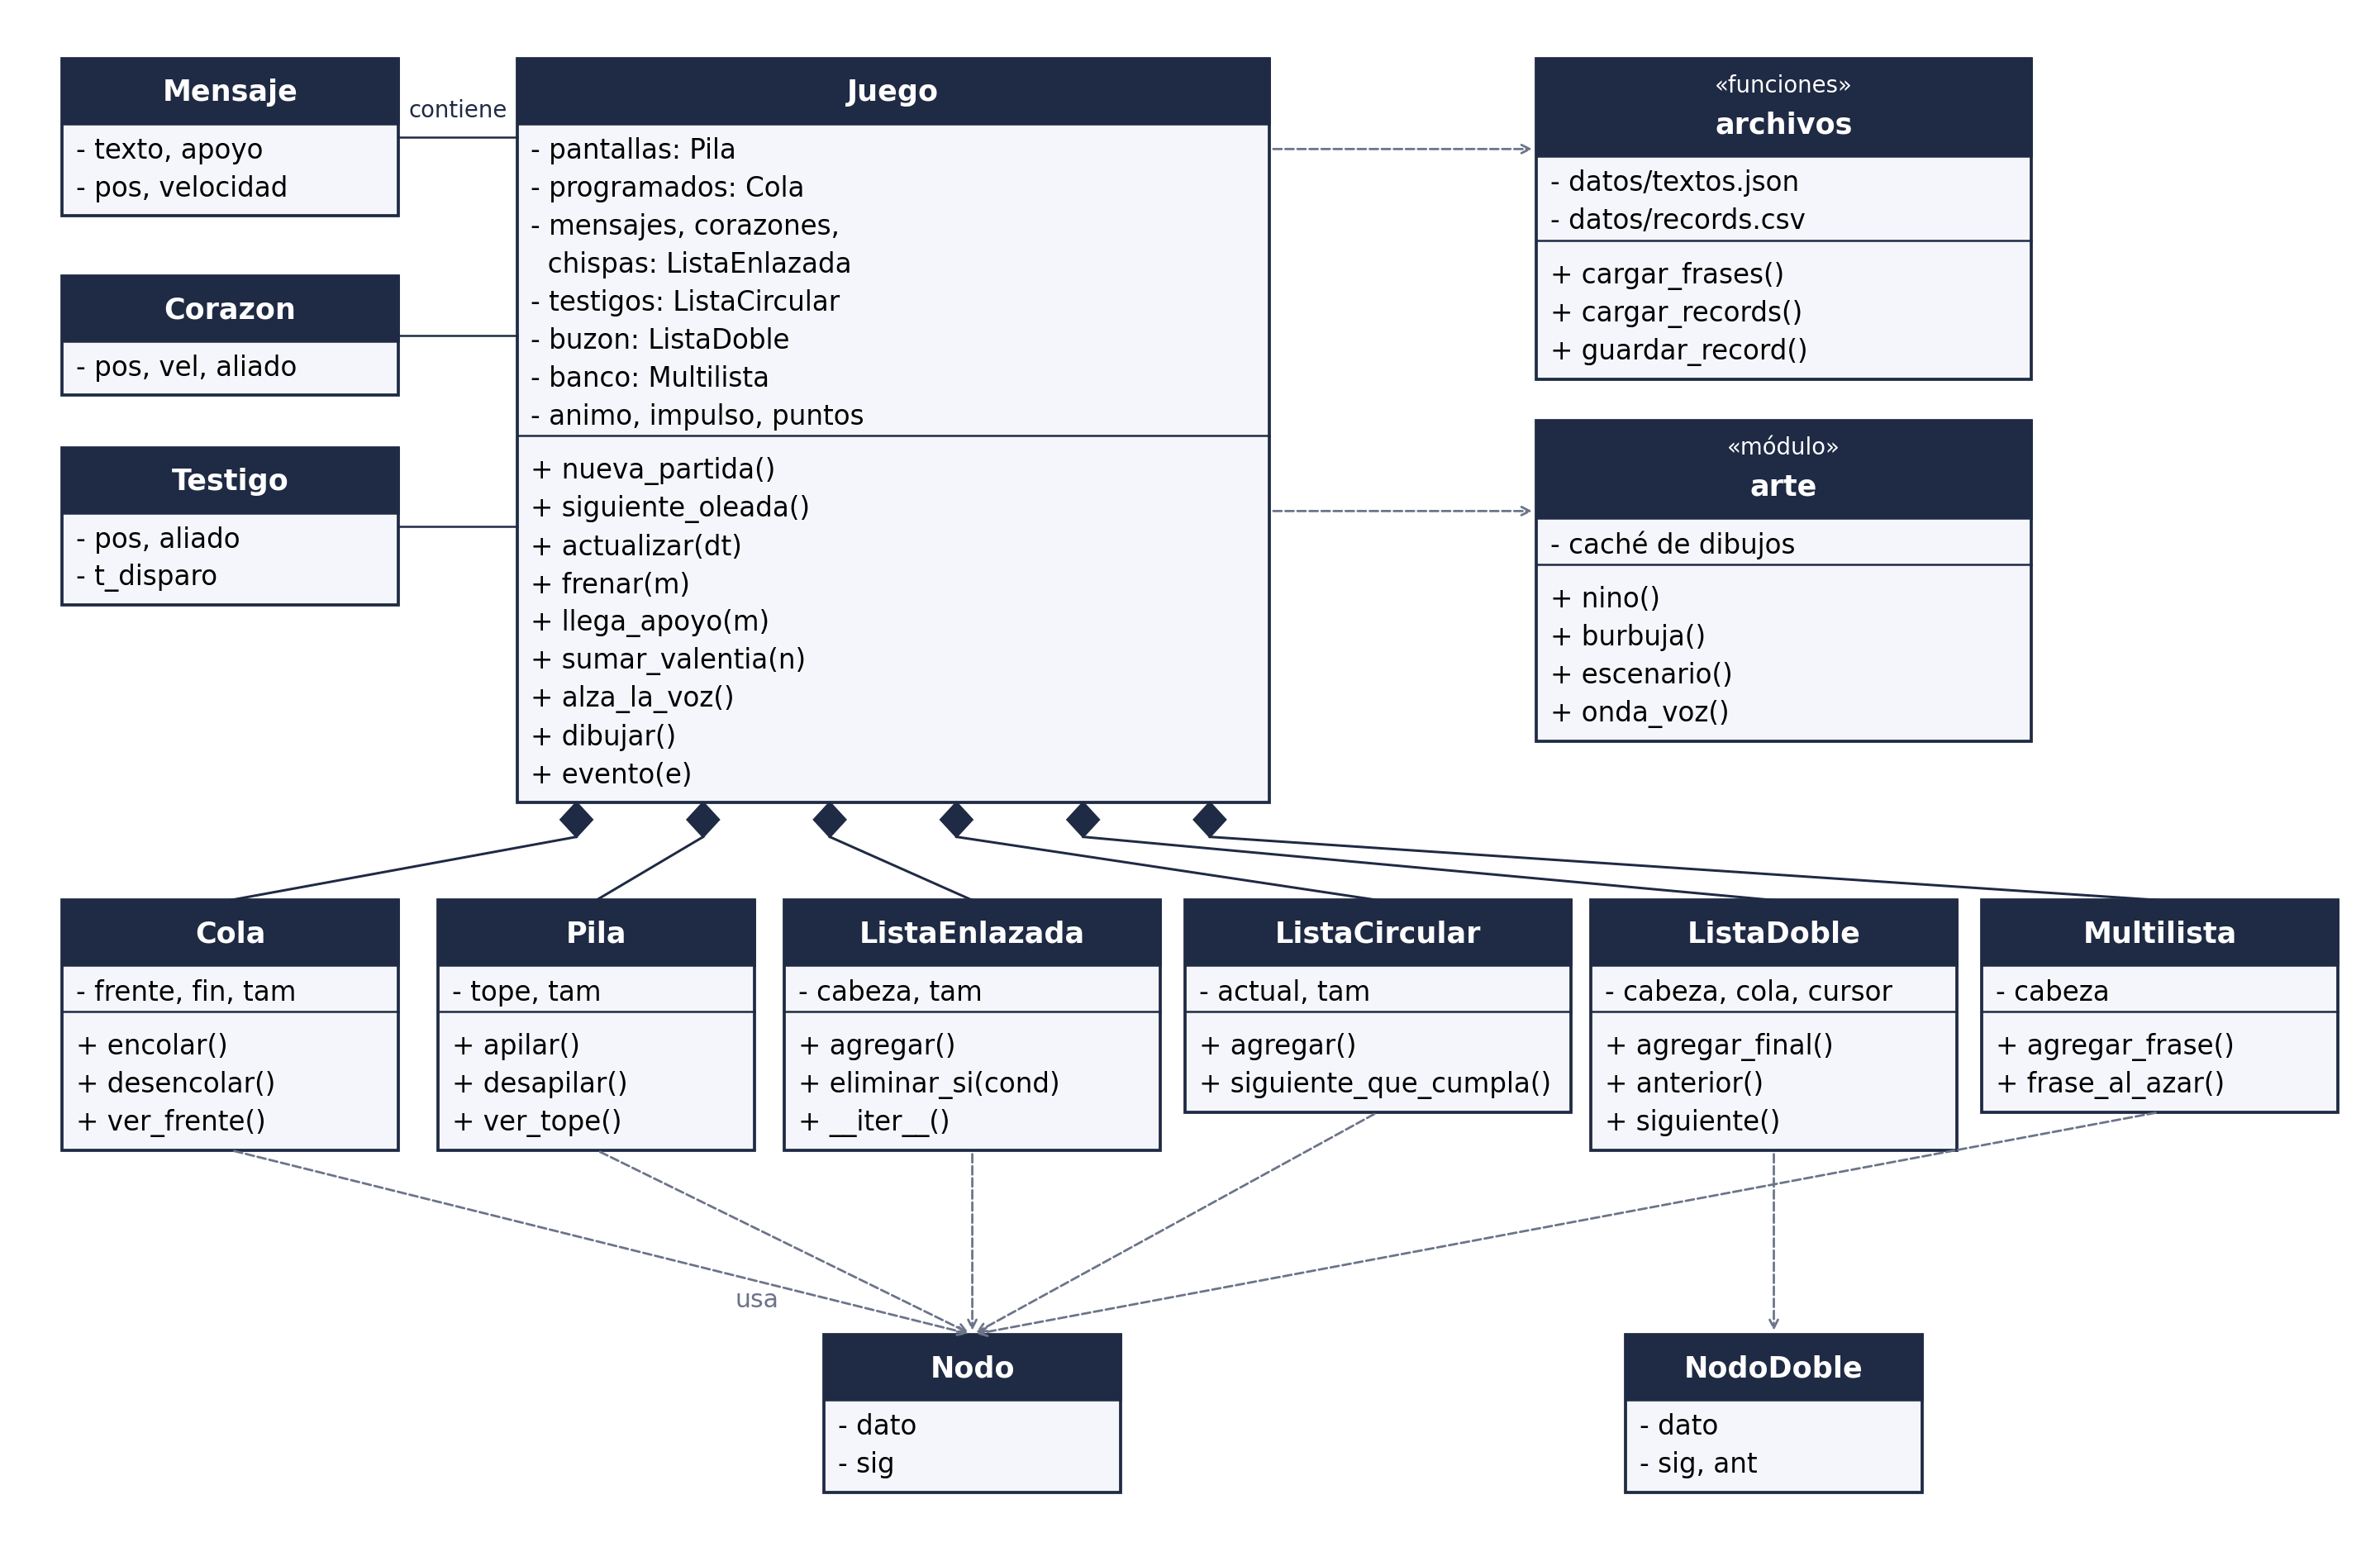
\includegraphics[width=0.9\textwidth]{figuras/diagrama_clases_final.png}
\caption{Class diagram of the final version.}
\end{figure*}

Table IV summarizes what each structure is for and why it was chosen. The cycle of one frame, in the actualizar (update) method, always follows the same order. First, messages whose time has come move from the queue to the linked list; then the player, hearts and messages move, and collisions are checked. Messages that are stopped or reach Sam are not deleted at that moment: they are marked, and at the end of the frame eliminar\_si removes them from the list in a single pass. This way a list is never modified while it is being traversed.

\begin{table*}[!htbp]
\centering
\caption{Data structures and their use in the game}
\footnotesize
\begin{tabularx}{\textwidth}{|l|X|X|}
\hline
\textbf{Structure} & \textbf{Use} & \textbf{Why this structure} \\ \hline
Queue & Messages scheduled for the wave (second, type and angle). & They leave in the order they were scheduled (FIFO). \\ \hline
Stack & Open screens: menu, game, pause, help, high scores and end. & Going back returns to the last screen opened (LIFO). \\ \hline
Linked list & Messages, hearts, sparks and notices on screen. & Nodes are removed from any position in a single pass. \\ \hline
Circular list & The eight bystanders around Sam. & Courage passes to the next neighbor and, after the last one, the traversal returns to the first. \\ \hline
Doubly linked list & Mailbox with the supportive messages that reached Sam. & It is browsed forward and backward with the arrow keys. \\ \hline
Multilist & Phrase bank: 11 categories, each with its own list (59 bullying and 36 supportive). & The category is looked up and only its sublist is traversed. \\ \hline
Files & textos.json (phrases) and records.csv (top five scores). & Data is kept after closing the program and phrases can be edited without touching the code. \\ \hline
\end{tabularx}
\end{table*}

\subsection{Technology Environment}

The game is written in Python 3 with pygame-ce 2.5, the version of pygame maintained by its community \cite{ref10}. Python is the language the whole team knows, and in it data structures read almost like pseudocode \cite{ref11}. pygame-ce handles the window, drawing, sound and keyboard and mouse input, and it is faster to learn than a full engine. Characters, the ten settings, bubbles and icons are drawn with simple shapes at three times their size and scaled down with smoothing; sounds are generated as waves on the fly. That is why the game does not depend on external images or audio. The code was written in Visual Studio Code and the report in LaTeX with the IEEE template.

\subsection{Project Management}

The team worked as the company Nodo Sano Studios. Felipe Ríos was in charge of management; Josue Salas, code and design; Gustavo Parody, documentation; Camilo Meriño, testing, and Avid Avila, the interface and user experience. A simplified Scrum was followed, with one-week sprints that began with a short meeting. Tasks were tracked on a Trello board with the columns Backlog, This week, In progress, In review and Done, and each card had an owner, a role label and a due date.

\subsection{Evolution of the Prototype}

The first deliverable was a prototype of about 370 lines with three waves and four structures. For the final deliverable the mechanics of the group's JavaScript version were brought to Python: the boost and the ``\textexclamdown{}Alza la voz!'' wave, the bystanders, the mailbox, the settings and the boss. A first complete version reached about 4,600 lines, with upgrade cards, several enemy types and two extra modes. The team decided to cut it down: five people had to be able to explain all the code in the individual exam, and those pieces did not change the central idea of the game. The final version keeps the mechanics that teach something and brings juego.py and estructuras.py down to 1,056 lines; the drawing code, arte.py, takes another 816. The Arduino controller and the background music were left out.

\subsection{Use of Artificial Intelligence Tools}

Claude (Anthropic) was used to compare game concepts at the start, to generate and review code, for the drawing-by-code layer and as support in writing this report. The team ran and fixed the code, decided which mechanics stayed in the final version and looked up each reference in its original source. The contribution of AI is estimated at about 35 \%, concentrated at the start of the project and in getting the initial ideas working; in later stages it was only a support.

\section{Results}

\subsection{Final Version of the Game}

Fig. 2 shows the menu and Fig. 3 a game in the fifth wave (Physical education): Sam in the center, the bystanders around him and the faces of those who already help at the top. When Sam loses mood the setting turns blue and cold; when a supportive message arrives, Sam jumps and his aura lights up. Fig. 4 shows the ``\textexclamdown{}Alza la voz!'' wave during the final boss and Fig. 5 the high contrast mode, in which bullying and support can still be told apart by shape.

\begin{figure}[!htbp]
\centering
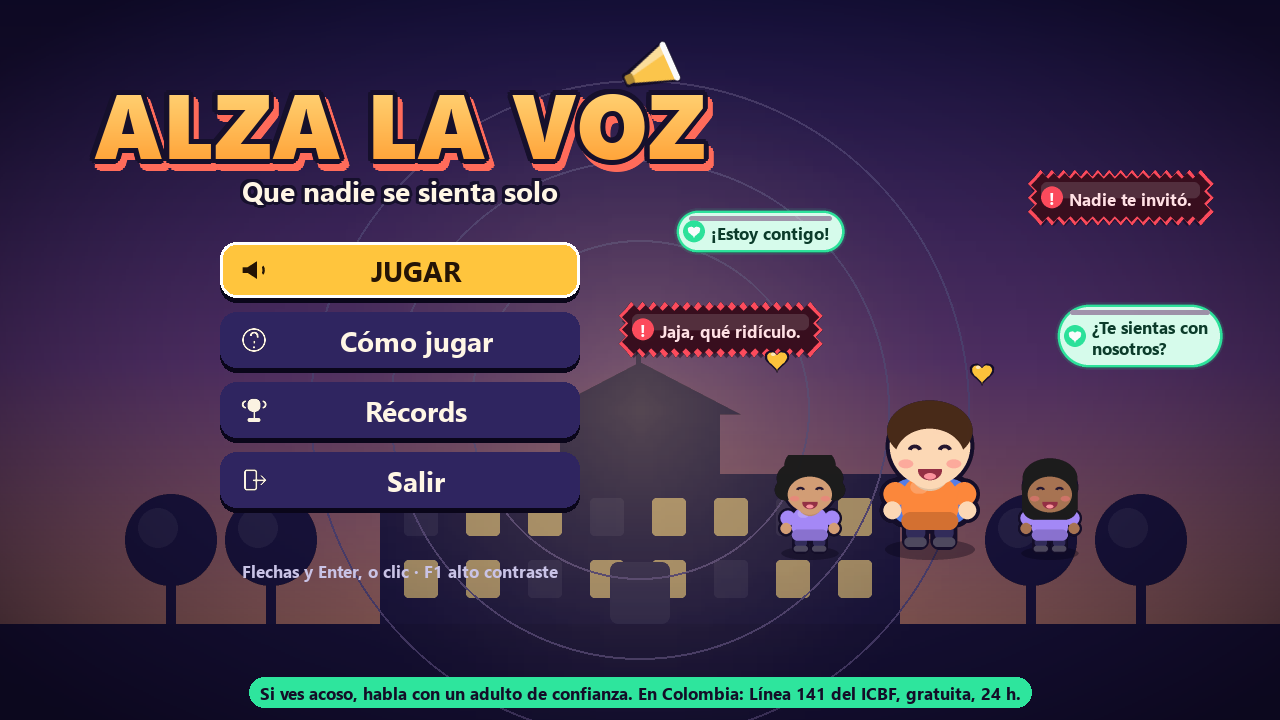
\includegraphics[width=\columnwidth]{figuras/01_menu.png}
\caption{Main menu.}
\end{figure}

\begin{figure}[!htbp]
\centering
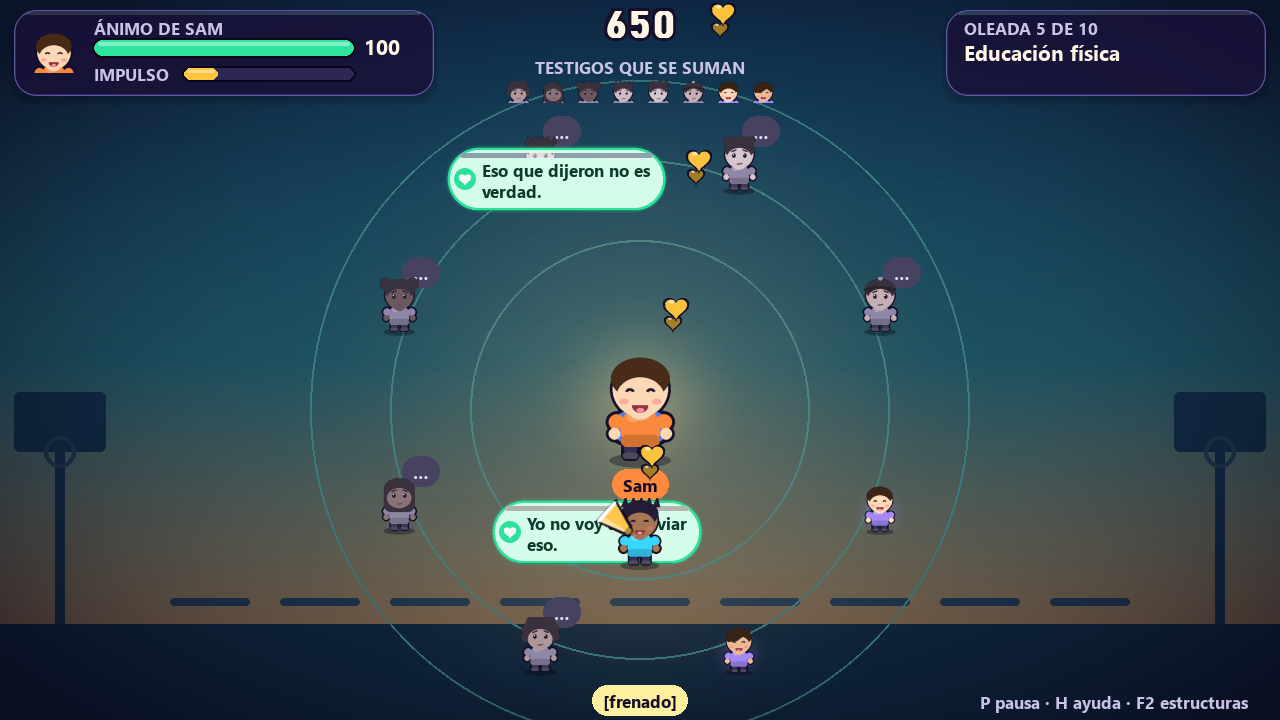
\includegraphics[width=\columnwidth]{figuras/03_oleada05.png}
\caption{Game in wave 5: grey bystanders who watch and purple ones who help.}
\end{figure}

\begin{figure}[!htbp]
\centering
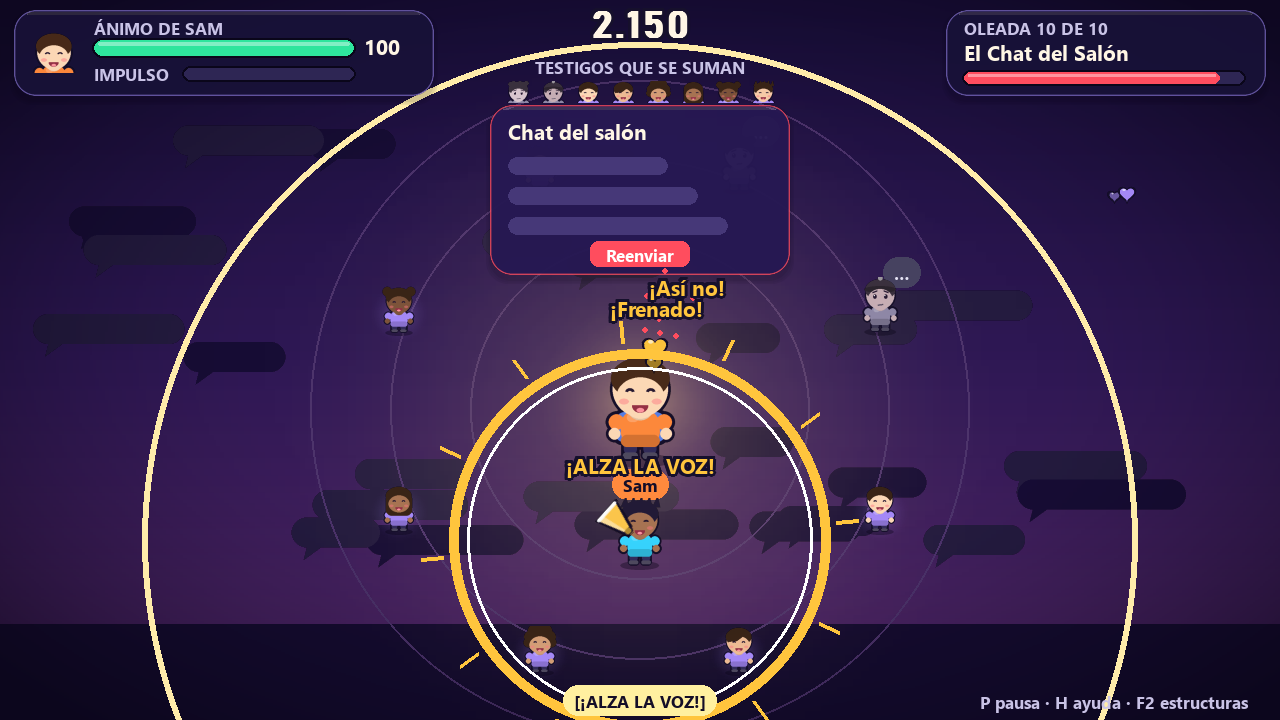
\includegraphics[width=\columnwidth]{figuras/04_alza_la_voz.png}
\caption{``\textexclamdown{}Alza la voz!'' wave against the boss El Chat del Salón (the class chat).}
\end{figure}

\begin{figure}[!htbp]
\centering
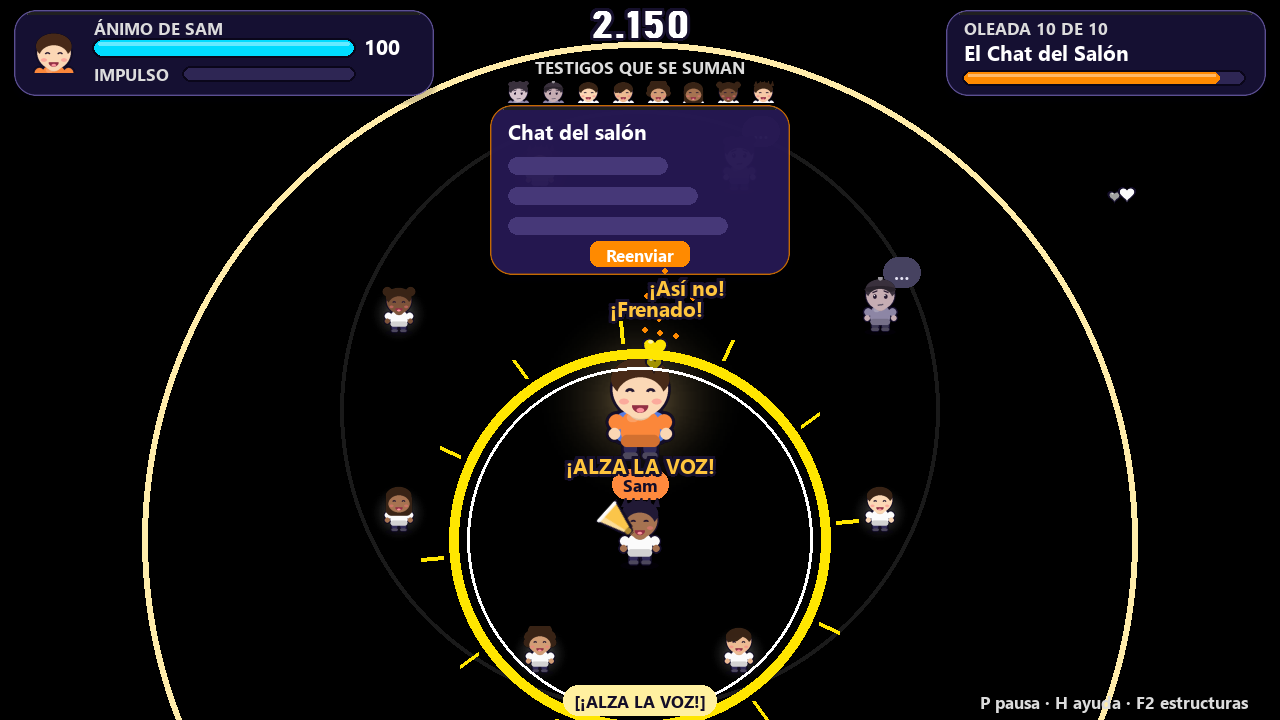
\includegraphics[width=\columnwidth]{figuras/06_alto_contraste.png}
\caption{High contrast mode.}
\end{figure}

\subsection{Automated Tests}

The script pruebas/test\_estructuras.py checked each structure separately: the order of the queue and the stack, deletion in the linked list at the start, middle and end, a full turn of the circular list, the cursor limits of the doubly linked list and the category lookup in the multilist. All six tests passed. The script pruebas/simulacion.py played complete games with no human input (Table V): in the first three, the script reached the tenth wave and beat the boss.

\begin{table*}[!htbp]
\centering
\caption{Automated games}
\footnotesize
\begin{tabularx}{\textwidth}{|l|X|X|X|X|}
\hline
\textbf{Game} & \textbf{Result} & \textbf{Stopped} & \textbf{Support} & \textbf{Allies} \\ \hline
Normal & Victory (wave 10) & 135 & 34 & 8 \\ \hline
Sam never falls & Victory (wave 10) & 136 & 31 & 8 \\ \hline
Random keys, Sam never falls & Victory (wave 10) & 143 & 26 & 8 \\ \hline
Idle with 8 allies (20 runs) & Defeat, wave 6 (5 to 8) & 44 & 32 & 8 \\ \hline
Idle, no help (20 runs) & Defeat, wave 2 (1 to 6) & 2 & 7 & - \\ \hline
\end{tabularx}
\end{table*}

The last two rows were used to tune the balance. In an earlier version allies shot every 1.8 s at any message and the game almost played itself. Now they join every 10 points of courage and shoot every 3.5 s, only at what is less than 200 pixels from Sam. The last two rows are medians of 20 runs with different seeds (pruebas/balance\_y\_rendimiento.py). With all eight allies given and an idle player, Sam fell between the fifth and the eighth wave, and no run ended in victory.

The simulation also tried wrong inputs. A test name with symbols, an emoji and 23 characters was saved as ``Botñ 1234567'', and the game started and played with a damaged high score file and without the phrase file. All runs had zero errors. With 40 messages and 150 sparks on screen, updating and drawing one frame took a median of 1.4 ms and 3.7 ms at the 95th percentile, with no window; at 60 frames per second the limit is 16.7 ms.

\subsection{Usability Test}

For the test with people, a moderated testing protocol was prepared following Moran \cite{ref12}: each participant plays without prior instructions while a team member watches and takes notes, with four tasks (understanding what to do in the menu, stopping a bullying message and letting a supportive one through, using ``\textexclamdown{}Alza la voz!'' and browsing the mailbox during pause), and at the end answers the System Usability Scale (SUS) \cite{ref13}, ten questions scored from 0 to 100. That test could not be run before this deliverable, so this report contains no data from people.

Instead, a preliminary evaluation was run with pruebas/usabilidad\_bots.py, in which five bot profiles played using only simulated keyboard and mouse input, through the same path a person uses (Table VI). The first run had no errors, but the Novice and Trigger-happy profiles, which also shot supportive messages, won the game, because stopping a supportive message only cost 50 points. The game was not punishing the very confusion it aims to correct. Stopping a supportive message now also takes 8 of Sam's mood and 25 of the boost. Table VI shows the run after the change: the two profiles that do not tell messages apart lose in the third wave and the one that aims only at bullying still wins. The bots check that the game responds well to each kind of player; whether a student understands the rule in under a minute (RNF2) remains to be tested with people.

\begin{table*}[!htbp]
\centering
\caption{Preliminary evaluation with five bot profiles}
\footnotesize
\begin{tabularx}{\textwidth}{|l|X|X|X|X|}
\hline
\textbf{Profile} & \textbf{How it plays} & \textbf{Result} & \textbf{First bullying stopped} & \textbf{Shots at support} \\ \hline
Expert & Aims only at bullying and uses the boost & Victory (wave 10) & 5.5 s & 26 \\ \hline
Novice & Aims late and badly; opens help & Defeat (wave 3) & 3.6 s & 14 \\ \hline
Trigger-happy & Shoots at everything that comes close & Defeat (wave 3) & 5.6 s & 15 \\ \hline
Random keys & Mashes keys, pause, F1, F2 and Q & Restarts in wave 1 & 5.0 s & 54 \\ \hline
Idle & Touches nothing & Defeat (wave 1) & Never & 0 \\ \hline
\end{tabularx}
\end{table*}

\section{Conclusions}

Alza la Voz met the functional requirements and the non-functional ones that could be measured with automated tests; RNF2 depends on the user test. The game has a random component in the order, type and direction of messages, and a skill component in aiming without hitting supportive messages and in choosing when to use the boost. For accessibility it has high contrast and captions. At no point does it ask questions: the lesson comes from what happens to Sam after each decision. The six structures have a visible role in the game, and the circular list of bystanders represents the central idea of the project, that courage spreads.

The automated tests showed a stable game with room to spare in performance, but they say nothing about learning. A script that wins every game does not prove that a student will intervene upon seeing bullying at school. The test with people will measure whether the game is understood; measuring a change in behavior would require a study like those of Ferreira et al. \cite{ref3} or Özer and Bilgin \cite{ref9}, with control groups and follow-up, which is beyond the scope of this course.

There are other limitations. The game has no background music, only sound effects, and the Arduino controller planned in the first deliverable was not built. The phrases are in Spanish and written for Colombia. A later version could measure with users whether shots at supportive messages drop between the first and the third game, which would indicate that the player learns to recognize bullying disguised as a joke. A classroom mode could also be added in which the teacher sees the phrases that reached the mailbox and discusses them with the group.

\FloatBarrier

\begin{thebibliography}{10}
\bibitem{ref1} UNESCO, \textit{Behind the Numbers: Ending School Violence and Bullying}. Paris, France: UNESCO, 2019.
\bibitem{ref2} OECD, ``PISA 2022 Results (Volume I and II) -- Country Notes: Colombia,'' OECD Publishing, Paris, France, 2023. [Online]. Available: \url{https://www.oecd.org/en/publications/pisa-2022-results-volume-i-and-ii-country-notes_ed6fbcc5-en/colombia_dd5f34d9-en.html}. Accessed: Oct. 3, 2026.
\bibitem{ref3} P. C. Ferreira, A. M. Veiga Simão, A. Paiva, C. Martinho, R. Prada, and J. Rocha, ``Serious game-based psychosocial intervention to foster prosociality in cyberbullying bystanders,'' \textit{Psychosocial Intervention}, vol. 31, no. 2, pp. 83--96, 2022, doi: 10.5093/pi2022a5.
\bibitem{ref4} A. Calvo-Morata, C. Alonso-Fernández, M. Freire, I. Martínez-Ortiz, and B. Fernández-Manjón, ``Serious games to prevent and detect bullying and cyberbullying: A systematic serious games and literature review,'' \textit{Computers \& Education}, vol. 157, 2020, Art. no. 103958, doi: 10.1016/j.compedu.2020.103958.
\bibitem{ref5} A. Calvo-Morata, C. Alonso-Fernández, M. Freire, I. Martínez-Ortiz, and B. Fernández-Manjón, ``Creating awareness on bullying and cyberbullying among young people: Validating the effectiveness and design of the serious game Conectado,'' \textit{Telematics and Informatics}, vol. 60, 2021, Art. no. 101568, doi: 10.1016/j.tele.2021.101568.
\bibitem{ref6} Y. Achab Moukram, A. Manzano-León, J. M. Rodríguez-Ferrer, J. Rodríguez-Moreno, and J. M. Aguilar-Parra, ``A systematic review of gamification as a playful strategy to prevent bullying,'' \textit{Environment and Social Psychology}, vol. 7, no. 2, 2023, doi: 10.18063/esp.v7.i2.1566.
\bibitem{ref7} L. Wei, M. Schmierbach, B. Liu, J. Kang, C. Chen, F. E. Dardis, R. Tan, and O. Cohen, ``Amplifying player experience to facilitate prosocial outcomes in a narrative-based serious game,'' \textit{Media and Communication}, vol. 13, 2025, Art. no. 8637, doi: 10.17645/mac.8637.
\bibitem{ref8} Q. Chen, Z. Lu, B. Liu, Q. Xiao, and K. L. Chan, ``Effectiveness of digital game-based GISCC program on cyberbullying prevention among Chinese adolescents,'' \textit{Child Abuse \& Neglect}, vol. 161, 2025, Art. no. 107293, doi: 10.1016/j.chiabu.2025.107293.
\bibitem{ref9} \.I. Ö. Özer and M. Bilgin, ``Enhancing active bystander intervention in bullying through a web-based visual novel: Preliminary findings from a randomized trial,'' \textit{International Journal of Bullying Prevention}, published online, 2026, doi: 10.1007/s42380-026-00353-5.
\bibitem{ref10} pygame-ce, ``Pygame Community Edition documentation.'' [Online]. Available: \url{https://pyga.me/docs/}. Accessed: Oct. 3, 2026.
\bibitem{ref11} M. T. Goodrich, R. Tamassia, and M. H. Goldwasser, \textit{Data Structures and Algorithms in Python}. Hoboken, NJ, USA: Wiley, 2013.
\bibitem{ref12} K. Moran, ``Usability testing 101,'' Nielsen Norman Group, 2019. [Online]. Available: \url{https://www.nngroup.com/articles/usability-testing-101/}. Accessed: Nov. 22, 2026.
\bibitem{ref13} J. Brooke, ``SUS: A `quick and dirty' usability scale,'' in \textit{Usability Evaluation in Industry}, P. W. Jordan, B. Thomas, B. A. Weerdmeester, and I. L. McClelland, Eds. London, U.K.: Taylor \& Francis, 1996, pp. 189--194.
\end{thebibliography}
\end{document}
